\section{FUSE}
\gls{FUSE} is a library that provides an interface to create filesystems in userspace rather than in kernel space which is otherwise often considered the standard when writing commercial filesystems\,\cite{Libfuse2021}. The reason to implement a filesystem in kernel space is that it leads to faster system calls than when writing a filesystem in userspace. However, while filesystems written with \gls{FUSE} are generally slower than \mbox{kernel-based} filesystems, using \gls{FUSE} simplifies the process of creating filesystems. macFUSE is a port of \gls{FUSE} that operates on Apple's macOS operating system and it extends the \gls{FUSE} \gls{API}\,\cite{HomeMacFUSE}. macFUSE provides an \gls{API} for C and Objective C.
% TODO: MAYBE add about this "If you use these extensions, then how is it portable to \mbox{non-MAC} systems?". Cannot find anything online though

Figure~\ref{fig:fuse_desc} presents an overview how \gls{FUSE} works. \gls{FUSE} consists of a kernel space part and a userspace part that perform different tasks\,\cite{vangoorFUSENotFUSE2017}. The kernel part of \gls{FUSE} operates with the \gls{VFS} which is a layer in both the Linux kernel and the macOS kernel that exposes a filesystem interface for userspace applications\,\cite{goochOverviewLinuxVirtual, singhMacOSInternals2006}. The \gls{VFS} interface is independent of the underlying filesystem and is an abstraction of the underlying filesystem operations which can be used on any filesystem the \gls{VFS} supports. The userspace part of \gls{FUSE} communicates with the kernel space part through a block device. Operations on a mounted \gls{FUSE} filesystem are sent to the \gls{VFS} from the user application, which is then sent to the kernel part of \gls{FUSE}. If needed, the operations are transmitted to the userspace part of \gls{FUSE} where the operation is handled and a response is sent back to the \gls{VFS} and the user application through the \gls{FUSE} kernel module. However, some actions can be handled by the \gls{FUSE} kernel module directly, such as if the file is cached in the kernel part of \gls{FUSE}\,\cite{vangoorFUSENotFUSE2017}. The response is then sent back to the user application from the kernel module through the \gls{VFS}.

\begin{figure}[!ht]
	\begin{center}
	  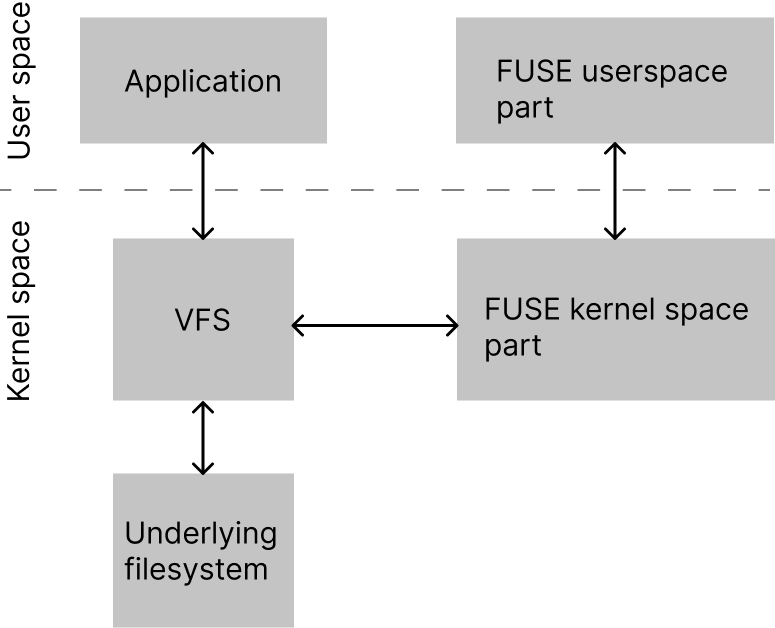
\includegraphics[width=0.5\textwidth]{figures/fuse_description.png}
	\end{center}
	\caption{Simple visualization of how \gls{FUSE} operations are executed}
	\label{fig:fuse_desc}
\end{figure}